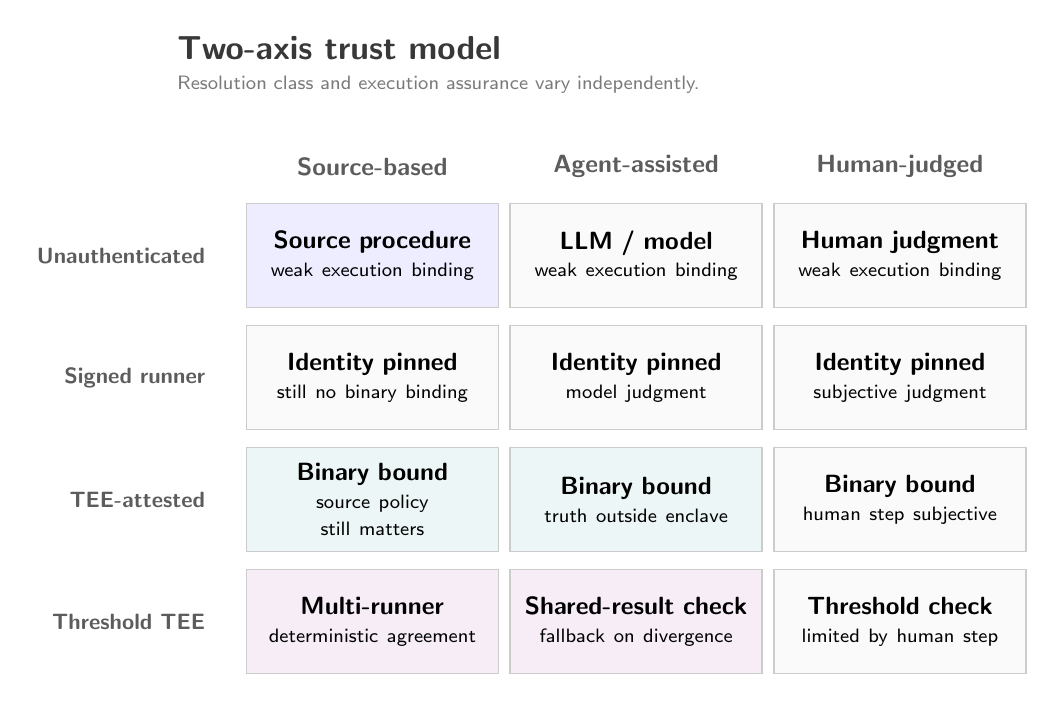
\begin{tikzpicture}[
  x=1cm, y=1cm,
  every node/.style={font=\sffamily},
  % ── Typography ───────────────────────────────────────────────────
  ftitle/.style={
    font=\sffamily\bfseries\fontsize{12.8pt}{13.8pt}\selectfont,
    text=black!78,
  },
  axislbl/.style={
    font=\sffamily\bfseries\fontsize{8.9pt}{9.9pt}\selectfont,
    text=black!68,
  },
  rowhead/.style={
    font=\sffamily\bfseries\fontsize{8.4pt}{9.4pt}\selectfont,
    text=black!64, align=right,
  },
  colhead/.style={
    font=\sffamily\bfseries\fontsize{8.6pt}{9.6pt}\selectfont,
    text=black!64, align=center,
  },
  small/.style={
    font=\sffamily\fontsize{7.3pt}{8.2pt}\selectfont,
    text=black!52, align=center,
  },
  % ── Grid cells ───────────────────────────────────────────────────
  cell/.style={
    draw=black!20, line width=0.55pt,
    minimum width=3.15cm, minimum height=1.32cm,
    text width=2.85cm,
    align=center, inner sep=5pt,
    font=\sffamily\fontsize{8.7pt}{10pt}\selectfont,
  },
  hi1/.style={cell, fill=blue!7},
  hi2/.style={cell, fill=teal!7},
  hi3/.style={cell, fill=violet!7},
  base/.style={cell, fill=black!2},
]

% ── Title ──────────────────────────────────────────────────────────
\node[anchor=west, ftitle] at (-0.05, 0.78) {Two-axis trust model};
\node[anchor=west, small] at (-0.05, 0.32) {Resolution class and execution assurance vary independently.};

% ── Column headers ─────────────────────────────────────────────────
\node[colhead] at (2.55, -0.72) {Source-based};
\node[colhead] at (5.90, -0.72) {Agent-assisted};
\node[colhead] at (9.25, -0.72) {Human-judged};

% ── Row headers ────────────────────────────────────────────────────
\node[rowhead, anchor=east] at (0.55, -1.85)  {Unauthenticated};
\node[rowhead, anchor=east] at (0.55, -3.40) {Signed runner};
\node[rowhead, anchor=east] at (0.55, -4.95)  {TEE-attested};
\node[rowhead, anchor=east] at (0.55, -6.50) {Threshold TEE};

% ── Row 1: Unauthenticated ────────────────────────────────────────
\node[hi1]  at (2.55, -1.85)  {\textbf{Source procedure}\\{\scriptsize weak execution binding}};
\node[base] at (5.90, -1.85)  {\textbf{LLM / model}\\{\scriptsize weak execution binding}};
\node[base] at (9.25, -1.85)  {\textbf{Human judgment}\\{\scriptsize weak execution binding}};

% ── Row 2: Signed runner ──────────────────────────────────────────
\node[base] at (2.55, -3.40) {\textbf{Identity pinned}\\{\scriptsize still no binary binding}};
\node[base] at (5.90, -3.40) {\textbf{Identity pinned}\\{\scriptsize model judgment}};
\node[base] at (9.25, -3.40) {\textbf{Identity pinned}\\{\scriptsize subjective judgment}};

% ── Row 3: TEE-attested ───────────────────────────────────────────
\node[hi2]  at (2.55, -4.95)  {\textbf{Binary bound}\\{\scriptsize source policy still matters}};
\node[hi2]  at (5.90, -4.95)  {\textbf{Binary bound}\\{\scriptsize truth outside enclave}};
\node[base] at (9.25, -4.95)  {\textbf{Binary bound}\\{\scriptsize human step subjective}};

% ── Row 4: Threshold TEE ──────────────────────────────────────────
\node[hi3]  at (2.55, -6.50) {\textbf{Multi-runner}\\{\scriptsize deterministic agreement}};
\node[hi3]  at (5.90, -6.50) {\textbf{Shared-result check}\\{\scriptsize fallback on divergence}};
\node[base] at (9.25, -6.50) {\textbf{Threshold check}\\{\scriptsize limited by human step}};

\end{tikzpicture}
